\documentclass[a4paper,11pt]{article}
\input{/home/tof/Documents/Cozy/latex-include/preambule_doc.tex}
\input{/home/tof/Documents/Cozy/latex-include/preambule_commun.tex}
\newcommand{\showprof}{show them}  % comment this line if you don't want to see todo environment
\setlength{\fboxrule}{0.8pt}
\fancyhead[L]{\fbox{\Large{\textbf{Lang 01}}}}
\fancyhead[C]{\textbf{Jeu de dés - constructions élémentaires}}
\newdate{madate}{10}{09}{2020}
%\fancyhead[R]{\displaydate{madate}} %\today
\fancyhead[R]{Première - NSI}
\fancyfoot[L]{\vspace{1mm}Christophe Viroulaud}
\AtEndDocument{\label{lastpage}}
\fancyfoot[C]{\textbf{Page \thepage/\pageref{lastpage}}}
\fancyfoot[R]{\includegraphics[width=2cm,align=t]{/home/tof/Documents/Cozy/latex-include/cc.png}}
\usepackage{tikz}
\begin{document}
\framebox{Quelles constructions élémentaires sont suffisantes pour écrire n'importe quel programme?}
\section{Python: un langage de haut-niveau}

\begin{itemize}
    \item développé par \emph{Guido van Rossum} fin 1989,
    \item interprété, c'est à dire que le programme est lu ligne après ligne par un \emph{interpréteur}.
\end{itemize}
\section{Constructions élémentaires}
\subsection{Jeu de dés}
Pour construire un tel programme il faut pouvoir:
\begin{itemize}
    \item Stocker la valeur du dé dans une \textbf{variable}.
    \item Demander à l'utilisateur d'\textbf{entrer} une valeur.
    \item \textbf{Répéter}:
          \begin{itemize}
              \item \textbf{Comparer} la valeur de l'utilisateur à celle du dé.
              \item Incrémenter le nombre d'essais.
          \end{itemize}
    \item \textbf{Afficher (sortir)} le nombre d'essais dans la console.
\end{itemize}
\subsection{Interpréteur}
Il lit le code source ligne par ligne et l'exécute. Il est possible d'écrire du code directement dans la console de l'interpréteur, mais on préférera souvent utiliser un \textbf{Environnement de Développement Intégré}.
\subsection{Variables}
\begin{center}
\begin{lstlisting}[language=Python  , xleftmargin=2em, xrightmargin=2em]
de1 = 3
\end{lstlisting}
\captionof{code}{Une variable est une boîte étiquetée}
\label{CODE}
\end{center}
\begin{center}
    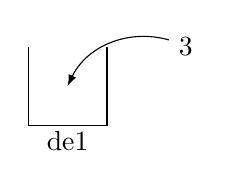
\begin{tikzpicture}
        \draw (0,1) -- (0,0) -- (1,0) -- (1,1);
        \node (3) at (2,1) {3};
        \node at (.5,-.2) {de1};
        \draw[->,>=latex] (3) to[bend right=40] (.5,.5);

    \end{tikzpicture}
    \captionof{figure}{Affectation}
\end{center}
\subsection{Entrée/Sortie}
\begin{center}
\begin{lstlisting}[language=Python  , xleftmargin=2em, xrightmargin=2em]
proposition =input("Choisir une valeur du dé: ")
\end{lstlisting}
\captionof{code}{Entrée: demander une valeur à l'utilisateur}
\begin{lstlisting}[language=Python  , xleftmargin=2em, xrightmargin=2em]
print(proposition)
\end{lstlisting}
\captionof{code}{Sortie: afficher une valeur dans la console}
\label{CODE}
\end{center}
\subsection{Comparaison}
\begin{center}
    \begin{lstlisting}[language=Python , basicstyle=\ttfamily, xleftmargin=2em, xrightmargin=2em]
if de1 == proposition:
    print("Gagné")
else:
    print("Perdu")
\end{lstlisting}
\captionof{code}{Le mot-clé \textbf{\texttt{if}} évalue la comparaison qui le suit.}
\end{center}
\subsection{Répétition}
\subsubsection{Boucle non bornée}
\begin{center}
    \begin{lstlisting}[language=Python , basicstyle=\ttfamily, xleftmargin=2em, xrightmargin=2em]
de1 = 3
proposition = 0
while de1 != proposition:
    proposition = int(input("Choisir: "))
\end{lstlisting}
\captionof{code}{Une boucle non bornée (\textbf{\texttt{while}}) répète une instruction tant que la condition est vérifiée.}
    \end{center}
\subsubsection{Boucle bornée}
\begin{center}
\begin{lstlisting}[language=Python  , xleftmargin=2em, xrightmargin=2em]
for compteur in range(10):
    print(compteur)
\end{lstlisting}
\captionof{code}{Une boucle bornée (\textbf{\texttt{for}}) effectue un nombre d'\emph{itérations} déterminé.}
\label{CODE}
\end{center}
\subsection{Bibliothèque}
\begin{center}
    \begin{lstlisting}[language=Python , basicstyle=\ttfamily, xleftmargin=2em, xrightmargin=2em]
from random import randint
de1 = randint(1,6)
\end{lstlisting}
    \captionof{code}{La bibliothèque \textbf{\texttt{random}} permet de générer un nombre aléatoire.}
    \label{aleatoire}
    \end{center}
\end{document}